 \documentclass[a4paper,12pt]{article}
%%%%%%%%%%%%%%%%%%%%%%%%%%%%%%%%%%%%%%%%%%%%%%%%%%%%%%%%%%%%%%%%%%%%%%%%%%%%%%%%%%%%%%%%%%%%%%%%%%%%%%%%%%%%%%%%%%%%%%%%%%%%%%%%%%%%%%%%%%%%%%%%%%%%%%%%%%%%%%%%%%%%%%%%%%%%%%%%%%%%%%%%%%%%%%%%%%%%%%%%%%%%%%%%%%%%%%%%%%%%%%%%%%%%%%%%%%%%%%%%%%%%%%%%%%%%
\usepackage{eurosym}
\usepackage{vmargin}
\usepackage{amsmath}
\usepackage{multicol}
\usepackage{graphics}
\usepackage{epsfig}
\usepackage{framed}
\usepackage{subfigure}
\usepackage{fancyhdr}

\setcounter{MaxMatrixCols}{10}
%TCIDATA{OutputFilter=LATEX.DLL}
%TCIDATA{Version=5.00.0.2570}
%TCIDATA{<META NAME="SaveForMode" CONTENT="1">}
%TCIDATA{LastRevised=Wednesday, February 23, 2011 13:24:34}
%TCIDATA{<META NAME="GraphicsSave" CONTENT="32">}
%TCIDATA{Language=American English}

%\pagestyle{fancy}
\setmarginsrb{20mm}{0mm}{20mm}{25mm}{12mm}{11mm}{0mm}{11mm}
%\lhead{MA4413 2013} \rhead{Mr. Kevin O'Brien}
%\chead{Midterm Assessment 1 }
%\input{tcilatex}

\begin{document}

\begin{center}
       
\includegraphics[scale=0.60]{shieldtransparent2}
\end{center}

\begin{center}
\vspace{1cm}
\large \bf {FACULTY OF SCIENCE AND ENGINEERING} \\[0.5cm]
\normalsize DEPARTMENT OF MATHEMATICS AND STATISTICS \\[1.25cm]
\large \bf {END OF SEMESTER EXAMINATION} \\[1.5cm]
\end{center}

\begin{tabular}{ll}
MODULE CODE: MA4413 & SEMESTER: Autumn 2013\\[1cm]
MODULE TITLE: Statistics for Computing & DURATION OF EXAM: 2.5 hours \\[1cm]
LECTURER: Kevin O'Brien & GRADING SCHEME: 100 marks\\
 & \phantom{GRADING SCHEME:} \footnotesize {70\% of total module marks}   \\[0.8cm]
EXTERNAL EXAMINER: Prof. Brendan Murphy & \\[1cm]
\\[1cm]
\end{tabular}
\begin{center}
{\bf INSTRUCTIONS TO CANDIDATES}
\end{center}

{\noindent \\ This paper is comprised of five questions, each worth 25 marks. Attempt any four questions.
\\ Scientific calculators approved by the University of Limerick can be used. 
\\ Formula sheet and statistical tables are provided.
}
\normalsize
\newpage
%\section*{Attempt ALL questions}

\section*{Question 1 [25 Marks]}
%-----------------------------------%



\bigskip

%--------------------------------------------------------------------- %
%Question 1
%--------------------------------------------------------------------- %

\begin{itemize}
\item[(a)]  \textbf{\textit{Probability (6 Marks)}}\\
An electronics assembly subcontractor receives its entire supply of resistors from two suppliers. Company A provides 70\% of the subcontractor's resistors, while company B supplies the remainder. The additional information has also been made available:

\begin{itemize}
\item[{$\bullet$}] 2\% of the resistors provided by company A failed the final test;
\item[{$\bullet$}] 3\% of company B's resistors also fail the final test.
\end{itemize}
\noindent Answer the following questions:
\begin{itemize}
\item[(i)](3 Marks) What is the probability that a resistor fails the final test?
\item[(ii)](3 Marks)  What is the probability that a resistor fails the final test given that the resistor in question came from company A?
%\item[iii.](2 marks) What is the probability that a resistor that fails final test was supplied by company A?
\end{itemize}

\item[(b)] \textbf{\textit{Descriptive Statistics (5 Marks)}}\\
Consider the following data set of seven numbers:

\begin{center}
\textbf{\texttt{4, 18,  2,  7, 18,  3,  4 }}
\end{center}
% 4 Marks

\noindent For this sample, compute the following descriptive statistics:
\begin{itemize}
%\item[a.] (1 Mark) The median,
\item[(i)] (1 Mark) the mean,
\item[(ii)] (1 Mark) the median,
\item[(iii)] (2 Marks) the variance,
\item[(iv)] (1 Mark) the standard deviation.
\end{itemize}
\end{itemize}

\begin{itemize}
\item[(c)] \textbf{\textit{Discrete Random Variables (6 Marks)}}\\
 The probability distribution of discrete random variable $X$ is tabulated below. There are five possible outcome of $X$, i.e. 2, 5, 10, 15 and 25.
\begin{center}
\begin{tabular}{|c||c|c|c|c|c|}
\hline
$x_i$ & 2 &  5 & 10 & 15 & 25  \\ \hline
$P(x_i)$ & 0.25 & 0.25 & 0.15 & \mbox{ k }  & 0.10 \\ \hline
\end{tabular}
\end{center}

\begin{itemize}
\item[(i)] (1 Mark) Compute the value for $k$.
\item[(ii)] (2 Marks) Determine the expected value $E(X)$.
\item[(iii)] (2 Marks) Evaluate $E(X^2)$.
\item[(iv)] (1 Mark) Compute the variance of random variable $X$.
\end{itemize}
{
\normalsize
\textit{\textbf{Please turn over for the remaining sections of Question 1.}}
}
\newpage
\item[(d)]  \textbf{\textit{Sampling without Replacement (4 Marks)}}\\
An urn contains 10 disks, 6 white and 4 red.  Two disks are selected, without replacement, from the urn.  Calculate the following probabilities:
 
\begin{itemize}
\item[(i)] (2 Marks) at least one disk is white;
\item[(ii)] (2 Marks)  exactly one disk chosen is white.
%\item[(iii)] (3 marks)                Neither disk chosen is red
%\item[(iv)] (3 marks)             At most one disk chosen is red
\end{itemize}
 
\item[(e)]\textbf{\textit{Independent Events (4 Marks)}}\\ Suppose A and B are two events, with P(A), the probability that A occurs, equal to 0.4 and P(B), the probability that B occurs, equal to 0.5. You may assume that A and B are independent events.
\begin{itemize}
\item[(i)] (2 Marks) Calculate P(A $\cap$ B), the probability of both A and B occuring. %if A and B are independent events.
\item[(ii)] (2 Marks) Calculate P(A $\cup$ B), the probability of either A or B (or both) occuring.
%\item[i]               A and B are mutually exclusive events
\end{itemize}
\end{itemize}
%Progress 7/15
%\subsection*{Question 1c Discrete Random Variable [5 Marks]}
%\item[(d)]The probability distribute of discrete random variable $X$ is tabulated below. There are 5 possible outcome of $X$, i.e. 1, 2, 3, 4 and 5.
%{
%\large
%\begin{center}
%\begin{tabular}{|c||c|c|c|c|c|}
%\hline
%$x_i$  & 1 & 2 & 3 & 4 & 5  \\\hline
%$p(x_i)$ & 0.30 & 0.20 & 0.20 & 0.10 & 0.20 \\
%\hline
%\end{tabular}
%\end{center}
%}
%\begin{itemize}
%%\item[a.] (1 Mark) Compute the value of $k$.
%\item[(a)] (1 Mark) What is the expected value of X?
%\item[(b)] (1 Mark) Compute the value of $E(X^2)$,
%\item[(c)] (1 Mark) Compute the variance of $X$.
%\end{itemize}
%\end{itemize}
\newpage

%------------------------------------------------------------ %
% Question 2
% Poisson Binomial Exponential
% Poisson Approximation
%------------------------------------------------------------ %

\section*{Question 2 [25 Marks]} 
%\subsection*{Part 2A : Poisson Distribution }
\begin{itemize}
\item[(a)] \textbf{\textit{Probability Distributions (9 Marks)}}\\
Telephone calls arrive at a switchboard at the rate of 40 per hour.  Assume that the telecentre operators take 3 minutes to deal with a customer query.  Calculate the probability of :
\begin{itemize} 
\item[(i)] (3 Marks)                 2 or more calls arriving in any 3 minute period.
\item[(ii)] (2 Marks)               No phone calls arriving in a 3 minute period,
\item[(iii)] (3 Marks)              Exactly one phone call arriving in any 3 minute period,
\item[(iv)] (1 Marks)             What is the average and standard deviation of the number of phone calls arriving in a 3 minute? period.
\end{itemize}
%\noindent (When answering, justify your answer with workings, or by reference to an axiom, theorem or rule.)


\bigskip
%-----------------------------------%
%\subsection*{Question 2B Binomial Distribution [3 Marks] } % 12 Marks
% New Question On Binomial

\item[(b)] \textbf{\textit{Probability Distributions (8 Marks)}}\\
For a digital communication channel, the probability of a bit being received in error is $5\%$. Consider the case where 100 bits are transmitted. Answer the following questions.

\begin{itemize}
\item[(i)] (3 marks)	What is the probability that the number of bits received in error is 5?
\item[(ii)] (3 marks) What is the probability that the number of bits received in error is greater than 10?
\item[(iii)] (2 marks)	What is the probability that the number of bits received in error does not exceed 12?
\end{itemize}

%\noindent(When answering, justify your answer with workings, or by reference to an axiom, theorem or rule.)



\item[(c)] \textbf{\textit{Probability Distributions (5 Marks)}}\\ On average, six people per hour use an electronic teller machine during the prime shopping hours in a department store. Therefore it is assumed that the expected time until the next customer will arrive will be 10 minutes. You may assume that the distributions of waiting times can be described by the exponential probability distribution.

\begin{itemize}
\item[(i)] (3 Marks) What is the probability that at least 10 minutes will pass between the arrival of two customers?
\item[(ii)] (2 Marks) What is the probability that after a customer leaves, another customer does not arrive for at least 20 minutes?
%\item[(iii)] (2 Marks) What is the probability that a second customer arrives within 1 min after a first customer begins a banking transaction?
\end{itemize}
\item[(d)] \textbf{\textit{Poisson Approximation of the Binomial Distribution (3 Marks)}}
\begin{itemize}
\item[(i)] (2 Marks) Describe how the Poisson distribution can be used to approximate the binomial distribution.
\item[(ii)] (1 Mark) Explain the circumstances in which this approximation may be used in preference to the binomial distribution.
\end{itemize}
\end{itemize}




\newpage
%--------------------------------------------------------------------- %
%Question 3 Normal Probability Distribution
%--------------------------------------------------------------------- %
%Question 3 Inference Procedures
%--------------------------------------------------------------------- %
%Question 3 Accuracy Precision and Recall

\subsection*{Question 3 [25 marks]}

% Minor Alterations to this Question


\begin{itemize}
%--------------------------------- %
\item[(a)] \textbf{\textit{Normal Probability Distribution (8 Marks)}}\\
A well known IT retailer has determined that the number of computer accessories sold, on a weekly basis in its largest shop, is normally distributed with a mean of 1000 and standard deviation of 50.
\begin{itemize}
\item[(i)] (2 Marks) Estimate the proportion of weeks that the company will sell more than 950 products.

\item[(ii)] (3 Marks) Estimate the proportion of weeks that the company will sell less than 975 products.
\item[(iii)] (3 Marks) Estimate the proportion of weeks that the company will sell between 950
products and 1025 products?
\end{itemize}
%--------------------------------- %

\item[(b)] \textbf{\textit{Theory of Statistical Inference (6 Marks)}}\\Answer the following questions on the theory of statistical inference.
\begin{itemize}
\item[(i)] (2 Marks) What is a $p-$value?
\item[(ii)] (2 Marks) Briefly describe how $p-$value is used in hypothesis testing.
\item[(iii)] (1 Mark) What is meant by a ``Type I error"?
\item[(iv)] (1 Mark) What is meant by a ``Type II error"?
\end{itemize}
%--------------------------------- %
\bigskip

\item[(c)] \textbf{\textit{Confidence Intervals (4 Marks)}}\\
A press release for a broadband provider stated that $90\%$ percent of customers are very satisfied
with the standard of service. To test this claim, the local chamber of commerce surveyed 110 randomly selected customers. Among the sampled customers, 89 stated that they are very satisfied.


%Test the hypothesis that $90\%$ of all customers are very satisfied with their service. You may assume a significance level of 5\%.



\begin{itemize}
\item[(i)] (1 Mark) Compute the appropriate value for the standard error for a confidence interval.
\item[(ii)] (2 Marks) Compute the 95\% confidence interval for $\pi$, the true proportion.
%\item[iii] (2 marks) For the test statistic, determine the corresponding p-value.
\item[(iii)] (1 Mark) What is your conclusion for this claim made by the press release? Justify your answer.
\end{itemize}
%--------------------------------- %
\end{itemize}
{
\normalsize
\textit{\textbf{Please turn over for the remaining sections of Question 3.}}
}
%
\newpage
\begin{itemize}
%---------------------------------- %
\item[(d)] \textbf{\textit{ Inference Procedures with \texttt{R} (4 Marks)}}\\
Consider the following inference procedure performed on data set $X$.
\begin{center}
\begin{framed}
\begin{verbatim}
> shapiro.test(X)

        Shapiro-Wilk normality test

data:  X
W = 0.9619, p-value = 0.6671

\end{verbatim}
\end{framed}
\end{center}

\begin{itemize}
\item[(i)] (1 Mark) Describe what is the purpose of this statistical procedure.
\item[(ii)] (2 Marks) What are the null and alternative hypotheses?
\item[(iii)] (1 Mark) Write the conclusion that follows from the code output, displayed above.
\end{itemize}
\end{itemize}

%---------------------------------- %
\begin{itemize}
\item[(e)] \textbf{\textit{Graphical Procedures (3 Marks)}}
\begin{itemize}
\item[(i)] (2 Marks) The graph below depicts a normal probability plot. Describe what this plot is used for and how to interpret one.
\item[(ii)](1 Mark) What is your conclusion for the data used to construct the normal probability plot below?
\end{itemize}
\begin{center}
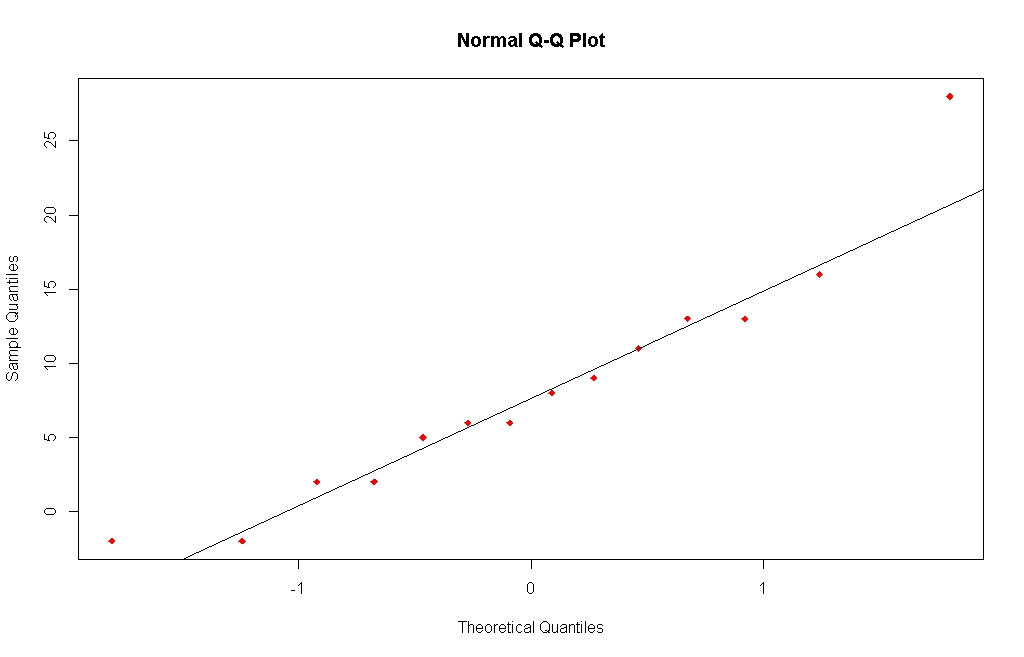
\includegraphics[scale=0.38]{10AQQplot}
\end{center}
\end{itemize}
%\end{document}

%\end{itemize}



%--------------------------------------------------------------------- %
%Question 4 

% Accuracy Precsion and Recall (7 Marks)
% Two Sample Hypothesis test for Sample Proportions (8 Marks)
% Confidence Interval (5 Marks)

%--------------------------------------------------------------------- %
\newpage
\section*{Question 4 [25 marks]}
%\subsection*{Question 4. (20 marks) }

\begin{itemize}
\item[(a)] \textbf{\textit{Binary Classification (6 Marks)}}\\
For following binary classification outcome table, calculate the following appraisal metrics.
\begin{itemize}	
\item[(i)] (1 Mark)	accuracy;
\item[(ii)] (1 Mark)	recall;
\item[(iii)] (1 Mark)	precision;
\item[(iv)] (1 Mark)	F-measure.
\end{itemize}	

\begin{center}
\begin{tabular}{|c|c|c|}
\hline  & \phantom{spa}Predict Negative\phantom{spa} & \phantom{spa}Predict Positive\phantom{spa} \\ 
\hline\phantom{spa} Observed Negative \phantom{spa}&	9530	&	10	\\ 
\hline \phantom{spa}Observed Positive\phantom{spa} & 	300	&	160	\\ 
\hline 
\end{tabular} 
\end{center}

\begin{itemize}	
\item[(v)] (2 Marks) Explain why the F-measure is considered a more informative measure of performance than the Accuracy score.

\end{itemize}
\item[(b)] \textbf{\textit{Inference Procedures (10 Marks)}}\\
Two IT training companies, \textit{XtraTech} and \textit{YourSkills}, offer an exam preparation course for a well-known computer industry certification. A study was carried out to compare the results from the most recent group of students from both companies.
\begin{itemize}
\item[$\bullet$]30 students from the \textit{XtraTech} course have completed the test. The average score for these students was 910 marks with a standard deviation of 48 marks.

\item[$\bullet$]25 students from the \textit{YourSkills} course have completed the test. Their average score was 950 marks with a standard deviation of 42 marks.
\end{itemize}

Test the hypothesis that the both sets of students perform equally well on average. You may use a significance level of 5\%. You may assume that both samples are normally distributed and have equal variance.
%\end{itemize}
\begin{itemize}
\item[(i)] (2 Marks) Formally state the null and alternative hypotheses for this procedure.
\item[(ii)] (2 Marks) Compute the point estimate for the difference in means of the results from both courses.
\item[(iii)] (2 Marks) Compute the appropriate value for standard error for this test. Clearly show your workings.
\item[(iv)] (2 Marks) Compute the test statistic.
\item[(v)] (2 Marks) What is your conclusion for this procedure?
\end{itemize}
{
\normalsize
\textit{\textbf{Please turn over for the remaining sections of Question 4.}}
}
\newpage
\item[(c)] \textbf{\textit{Inference Procedures (9 Marks)}}\\A study finds that $42\%$ of IT users out of a random sample of 450 in a large
community preferred one web browser to all others. In another large community, $34\%$ of IT users out of a random sample of 350 prefer the same web browser.

\begin{itemize}
\item[(i)] (2 Marks) Compute the point estimate for the difference in proportions of IT users who prefer this particular web browser.
\item[(ii)] (4 Marks) Compute a 95\% confidence interval for this difference in proportions.
\item[(iii)] (3 Marks) Based on this confidence interval, test the hypothesis that the proportion of IT users using this web browser is the same for both communities. State your null and alternative hypotheses clearly.
\end{itemize}

\end{itemize}

%------------------------------------------------------------------- %
% Question 5
% Huffman Coding
%------------------------------------------------------------------- %
\newpage
\subsection*{Question 5 [25 marks] }
\begin{itemize}
\item[(a)] \textbf{\textit{Huffman Coding (8 Marks)}}\\
A discrete memoryless source $X$ has five symbols $\{x_1,x_2,x_3,x_4,x_5\}$ with probabilities $P(x_1) = 0.45$ , $P(x_2) = 0.20$, $P(x_3) = 0.16$, $P(x_4) = 0.14$ and $P(x_5) = 0.05$.

\begin{itemize}
\item[(i)] (5 Marks) Construct a Huffman code for X.
\item[(ii)] (3 Marks) Calculate the efficiency of the code.
%\item[(iii)] (1 marks) Calculate the redundancy of the code.
\end{itemize}
\bigskip
\item[(b)] \textbf{\textit{Binary Channels (8 Marks)}}\\
Consider the binary channel in the figure below.
\begin{center}
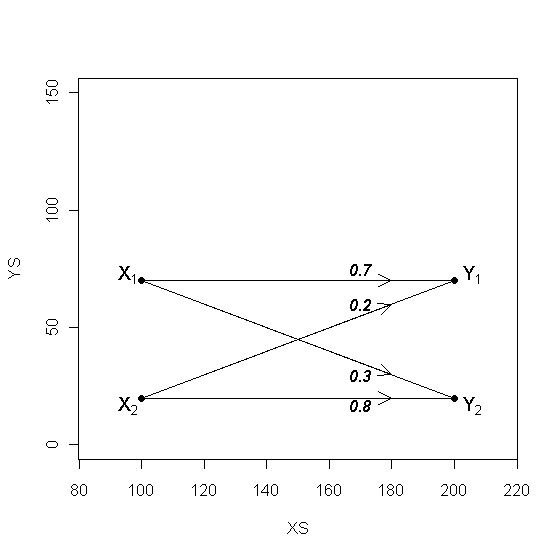
\includegraphics[scale=0.74]{10Bnet3}
\end{center}

\begin{itemize}
\item[(i)] (2 Marks) Determine the channel matrix of the channel
\item[(ii)] (3 Marks) Find $P(Y_1)$ and $P(Y_2)$ when $P(X_1) = 0.65$ and $P(X_2) = 0.35$.
\item[(iii)] (3 Marks) Find the joint probabilities $P(X_1,Y_1)$ and $P(X_2,Y_2)$ when $P(X_1) = 0.65$ and $P(X_2) = 0.35$.
\end{itemize}
\end{itemize}

{
\normalsize
\textit{\textbf{Please turn over for the remaining sections of Question 5.}}
}
%--------------------------------------------------------%
%  Question 5

%  Entropy
%  Huffman Coding
%--------------------------------------------------------%
\newpage
%\end{itemize}
\begin{itemize}
\item[(c)] \textbf{\textit{Rate of Information (5 Marks)}}\\
A high-resolution TV picture consists of about $2 \times 10^6$ picture elements (symbols) and 16
different brightness levels.\\
\newline
Pictures are repeated at a rate of 32 per second. All picture elements
are assumed to be independent, and all levels have equal likelihood of occurrence. 
\begin{itemize}
\item[(i)](5 Marks) Calculate the
average rate of information conveyed by this TV picture source.
\end{itemize}


\item[(d)] \textbf{\textit{Communication Channels (4 Marks)}}\\
The input source to a noisy communication channel is a random variable X over the
four symbols $\{a, b, c, d\}$. The output from this channel is a random variable Y over these same
four symbols. \\
\vspace{0.3cm}
\noindent 
The joint distribution of these two random variables is as follows:\\ \bigskip

\begin{center}
\begin{tabular}{|c|c|c|c|c|}
\hline
&x=a& x=b & x=c & x=d \\ \hline
y=a &1/8 &0 &0 & 0 \\ \hline
y=b &0 & 1/4& 1/8& 0 \\ \hline
y=c & 0&1/16 & 1/8 & 0\\ \hline
y=d & 1/16& 0& 0 & 1/4\\ \hline
\end{tabular}
\end{center}

\begin{itemize}
\item[(i)] (2 Marks) Write down the marginal distribution for $X$ and compute the marginal entropy $H(X)$.
\item[(ii)] (2 Marks) Write down the marginal distribution for $Y$ and compute the marginal entropy $H(Y )$.
%\item[(iii)] (2 Marks) What is the joint entropy $H(X, Y ) $ of the two random variables?
%\item[(iv)] (4 marks) What is the conditional entropy $H(Y|X)$?
%\item[(v)] (3 marks) What is the conditional entropy $H(X|Y)$?
%\item[(vi)] (3 marks) What is the mutual information $I(X;Y)$ between the two random variables?
\end{itemize}

\end{itemize}
\newpage






%\subsection*{Q6. Poisson Distribution (2 Marks) }  % 14 Marks
%Suppose that a telephone help-line receives 4 calls per hour during offices hours.
%\begin{itemize}
%\item[a.] (1 Mark) Compute the value of $m$ for a 30 minute period during office hours.
%\item[b.] (1 Mark) Compute the probability of the help-line getting exactly one call in a 30 minute period during office hours.
%\end{itemize}
%\bigskip
%\subsection*{Q7. Exponential Distribution (1 Mark)} % 15 Marks


%\begin{itemize}

%\item[a.] (1 Mark) Compute the value of $P(X \leq 482)$

%\end{itemize}
\newpage
\section*{Formulae}
\subsection*{Probability}
\begin{itemize}

\item Conditional probability:
\begin{equation*}
P(B|A)=\frac{P\left( A\text{ and }B\right) }{P\left( A\right) }.
\end{equation*}


\item Bayes' Theorem:
\begin{equation*}
P(B|A)=\frac{P\left(A|B\right) \times P(B) }{P\left( A\right) }.
\end{equation*}


\item Binomial probability distribution:
\begin{equation*}
P(X = k) = ^{n}C_{k} \times p^{k} \times \left( 1-p\right) ^{n-k}\qquad \left( \text{where}\qquad
^{n}C_{k} =\frac{n!}{k!\left(n-k\right) !}. \right)
\end{equation*}

\item Poisson probability distribution:
\begin{equation*}
P(X = k) =\frac{m^{k}\mathrm{e}^{-m}}{k!}.
\end{equation*}
\end{itemize}

\subsection*{Information Theory}

\begin{itemize}
\item $I(p) = - log_{2}(p) = log_{2}(1/p)$\\

\item $I(pq) = I(p) + I(q)$\\

\item $H = - \sum_{i=1}^{m}p_{i}\; log_{2}(p_{i})$\\

\item $E(L) = \sum_{i=1}^{m} l_{i} p_{i}$\\

\item $\mbox{Efficiency} = H / E(L)$\\

\item $I(X;Y) = H(X) - H(X|Y)$\\

\item $P(C[r]) = \sum_{j=1}^{m}P(C[r]|Y=d_{j} )P(Y=d_{j} )$

\item $R = rH(X) \mbox{      (b/second)}$
\end{itemize}

\newpage
\subsection*{Confidence Intervals}
{\bf One sample}
\begin{eqnarray*} S.E.(\bar{X})&=&\frac{\sigma}{\sqrt{n}}.\\\\
S.E.(\hat{P})&=&\sqrt{\frac{\hat{p}\times(100-\hat{p})}{n}}.\\
\end{eqnarray*}
{\bf Two samples}
\begin{eqnarray*}
S.E.(\bar{X}_1-\bar{X}_2)&=&\sqrt{\frac{\sigma^2_1}{n_1}+\frac{\sigma_2^2}{n_2}}.\\\\
S.E.(\hat{P_1}-\hat{P_2})&=&\sqrt{\frac{\hat{p}_1\times(100-\hat{p}_1)}{n_1}+\frac{\hat{p}_2\times(100-\hat{p}_2)}{n_2}}.\\\\
\end{eqnarray*}
\subsection*{Hypothesis tests}
{\bf One sample}
\begin{eqnarray*}
S.E.(\bar{X})&=&\frac{\sigma}{\sqrt{n}}.\\\\
S.E.(\pi)&=&\sqrt{\frac{\pi\times(100-\pi)}{n}}
\end{eqnarray*}
{\bf Two large independent samples}
\begin{eqnarray*}
S.E.(\bar{X}_1-\bar{X}_2)&=&\sqrt{\frac{\sigma^2_1}{n_1}+\frac{\sigma_2^2}{n_2}}.\\\\
S.E.(\hat{P_1}-\hat{P_2})&=&\sqrt{\left(\bar{p}\times(100-\bar{p})\right)\left(\frac{1}{n_1}+\frac{1}{n_2}\right)}.\\
\end{eqnarray*}
{\bf Two small independent samples}
\begin{eqnarray*}
S.E.(\bar{X}_1-\bar{X}_2)&=&\sqrt{s_p^2\left(\frac{1}{n_1}+\frac{1}{n_2}\right)}.\\\\
s_p^2&=&\frac{s_1^2(n_1-1)+s_2^2(n_2-1)}{n_1+n_2-2}.\\
\end{eqnarray*}
{\bf Paired sample}
\begin{eqnarray*}
S.E.(\bar{d})&=&\frac{s_d}{\sqrt{n}}.\\\\
\end{eqnarray*}
{\bf Standard deviation of case-wise differences}
\begin{eqnarray*}
s_d = \sqrt{ {\sum d_i^2 - n\bar{d}^2 \over n-1}}.\\\\
\end{eqnarray*}
{\bf Binary Classification}
\begin{itemize}
\item $F = 2 \times \frac{\mbox{precision} \times \mbox{recall}}{ \mbox{precision} + \mbox{recall}}$

\end{itemize}
\end{document}



\textbf{Description of the Experiment}
\begin{itemize}
\item Suppose we have two bags, each containing 2 marbles. 
\item One bag has 2 red marbles and
the other has a red marble and a yellow marble. 
You pick a bag at random and then pick
one of the marbles in that bag at random. 
\item When you look at the marble, it is red. 
You
now pick the second marble from that same bag.
\end{itemize} 
\textbf{Questions}
\begin{itemize}
\item[(a)](1 Mark)  Write down the sample space for this experiment, where the outcomes are the ordered pairs of drawn marbles.
\item[(b)](1 Mark) What is the probability that this marble
is also red? Select one of the options below, with a justification for your answer.
You may justify your answer by references to sample points.
\end{itemize}
\textbf{Options for part b}
\begin{center}
\begin{multicols}{4}
\begin{itemize}
\item[(i)] 1/4
\item[(ii)] 1/3
\item[(iii)] 2/3
\item[(iv)] 1/2
\end{itemize}
\end{multicols}
\end{center}
